\subsubsection{K-Way Mergesort}
The idea of sequential K-Way Mergesort is to enhance the merging phase by enlarging to $K$ the number of runs that are fused at a time. This approach, designed in the context of external-memory model, aims at reducing the I/O-complexity of Mergesort by improving the memory space utilization~\cite{FERR}. 

We reuse this idea, but with different purposes, to get another parallel version of Mergesort: now, the objective is not to lower the I/O-complexity, but rather to improve the \textit{efficiency}, that is both to diminish the number of steps of the algorithm and to increase the number or computing processor at each step. An initialization phase takes place as in Mergesort: $S$ is scattered among the processes and it is locally sorted. With respect to Mergesort, the distribution phase needs to be modified. While in Mergesort, in each step, there were exactly many senders as many receivers ($\frac{\sharp senders}{\sharp receivers} = 1$), in K-Way Mergesort the number of senders is higher ( $\frac{\sharp senders}{\sharp receivers} = K - 1$, see figure~\ref{k-merge-dist}). In other words, in a specific step, a process may receive data from $K-1$ processes. This approach allows us to reduce $m$ with respect to Mergesort. The merging phase is performed locally by the processes that have received $K-1$ blocks of data during the step. From sequential K-Way Mergesort we know that the best way to implement the fusion of more than two runs is to use a Heap data structure~\cite{FERR}; since in our parallel context the merging phase is not modified, we re-adopt the same approach.

We notice that in K-Way Mergesort the average value of $T_i$ may be different from the one we obtained for Mergesort. This is may due both to a longer merging phase and to the potential conflicts that may arise on the interconnection structure when $K-1$ processes try to send data to the same specific process.

\begin{figure}[h]
        \centerline{
               \mbox{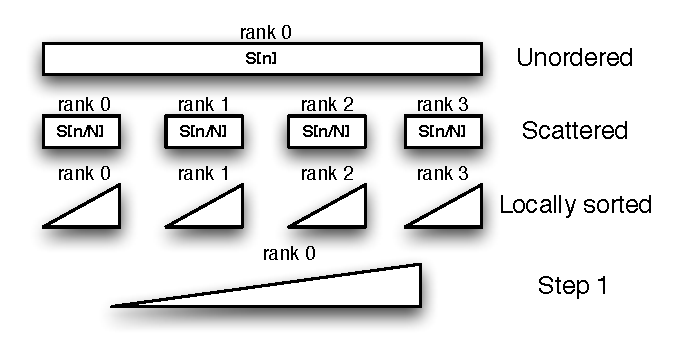
\includegraphics[scale=0.70]{kmerge-pict1}}
        }
        \caption{Parallel mergesort for $N = 4$, $K = 4$.}
        \label{k-merge-dist}
\end{figure}

\subsubsection*{Mapping virtual processors onto different cores} 
